%----------------------------------------------------------------------------------------
% PACKAGES AND DOCUMENT CONFIGURATIONS
%----------------------------------------------------------------------------------------

  \documentclass[12pt]{article}

  \usepackage{hyperref}
  \usepackage{fancyhdr} % Required for custom headers
  \usepackage{lastpage} % Required to determine the last page for the footer
  \usepackage{extramarks} % Required for headers and footers
  \usepackage[usenames,dvipsnames]{color} % Required for custom colors
  \usepackage{graphicx} % Required to insert images
  \usepackage{listings} % Required for insertion of code
  \usepackage{courier} % Required for the courier font
  \usepackage{lipsum} % Used for inserting dummy 'Lorem ipsum' text into the template
  \usepackage{wrapfig}
  \usepackage{color}
  \usepackage{lscape}

  \setlength\parindent{0pt} % Removes all indentation from paragraphs
  \renewcommand{\labelenumi}{\alph{enumi}.} % Make numbering in the itemize environment by letter rather than number (e.g. section 6)

  % Margins
  \topmargin=-0.4in
  \evensidemargin=0.2in
  \oddsidemargin=-0.2in
  \textwidth=7.0in
  \textheight=9.0in
  % \headsep=0.25in

  % \linespread{1.1} % Line spacing

  \definecolor{dkgreen}{rgb}{0,0.6,0}
  \definecolor{gray}{rgb}{0.5,0.5,0.5}
  \definecolor{mauve}{rgb}{0.58,0,0.82}
  \definecolor{greyish}{rgb}{0.96,0.96,0.96}

  \lstset{
    backgroundcolor=\color{greyish},   % choose the background color; you must add \usepackage{color} or \usepackage{xcolor}
    frame=tblr,
    numbers=left,                       % where to put the line-numbers; possible values are (none, left, right)
    numbersep=5pt,                   % how far the line-numbers are from the code
    numberstyle=\tiny\color{mygray}, % the style that is used for the line-numbers
    language=Ruby,
    aboveskip=3mm,
    belowskip=3mm,
    showstringspaces=false,
    columns=flexible,
    basicstyle={\footnotesize\ttfamily},
    numbers=none,
    numberstyle=\tiny\color{gray},
    keywordstyle=\color{blue},
    commentstyle=\color{dkgreen},
    stringstyle=\color{mauve},
    breaklines=true,
    breakatwhitespace=true
    tabsize=1
  }

  \begin{document}
  \begin{titlepage}

%----------------------------------------------------------------------------------------
% TITLE PAGE INFORMATION
%----------------------------------------------------------------------------------------
 \newcommand{\HRule}{\rule{\linewidth}{0.5mm}} % Defines a new command for the horizontal lines, change thickness here
  \begin{center} % Center everything on the page

  %----------------------------------------------------------------------------------------
  % HEADING SECTIONS
  %----------------------------------------------------------------------------------------
  \textsc{\large Faculty of Computers, Informatics and Microelectronics}\\[0.5cm]
  \textsc{\large Technical University of Moldova}\\[1.2cm] % Name of your university/college
  \vspace{35 mm}
  \textsc{\Large PAD}\\[0.5cm] % Major heading such as course name
  %\textsc{\large Laboratory work \#1-3}\\[0.5cm] % Minor heading such as course title
  \textsc{\large Laboratory work \# 2}\\[0.5cm] % Minor heading such as course title

  %----------------------------------------------------------------------------------------
  % TITLE SECTION
  %----------------------------------------------------------------------------------------
  \vspace{10 mm}
  \HRule \\[0.4cm]
  { \LARGE \bfseries Distributed systems  }\\[0.4cm] % Title of your document
  \HRule \\[1.5cm]

  %----------------------------------------------------------------------------------------
  % AUTHOR SECTION
  %----------------------------------------------------------------------------------------
      \vspace{30mm}

      \begin{minipage}{0.4\textwidth}
      \begin{flushleft} \large
      \emph{Authors:}\\
      \textbf{Petru \textsc{Negrei}} \\
      Victor \textsc{Vasilica}
      \end{flushleft}
      \end{minipage}
      ~
      \begin{minipage}{0.4\textwidth}
      \begin{flushright} \large
      \emph{Supervisor:} \\
      D. \textsc{Ciorba} % Supervisor's Name
      \end{flushright}
      \end{minipage}\\[4cm]

      \vspace{5 mm}
      % If you don't want a supervisor, uncomment the two lines below and remove the section above
      %\Large \emph{Author:}\\
      %John \textsc{Smith}\\[3cm] % Your name

      %----------------------------------------------------------------------------------------
      % DATE SECTION
      %----------------------------------------------------------------------------------------

      {\large September 2014}\\[3cm] % Date, change the \today to a set date if you want to be precise

      %----------------------------------------------------------------------------------------
      % LOGO SECTION
      %----------------------------------------------------------------------------------------

      %\includegraphics{Logo}\\[1cm] % Include a department/university logo - this will require the graphicx package

      %----------------------------------------------------------------------------------------

      \vfill % Fill the rest of the page with whitespace
      \end{center}
      \end{titlepage}

      % \newpage
      % \tableofcontents
      % \newpage

%----------------------------------------------------------------------------------------
% Introduction
%----------------------------------------------------------------------------------------

  \section{Introduction}

  \subsection{Topic}

  Building a distributed system.

  \subsection{Objective}

  Study of different transport protocols TCP/IP in order to build a application that contains collection of distributed data.

  \subsection{Generic requirements}

  \subsubsection{Task}

  \begin{itemize}
    \item Use UDP protocol for unicast and multicast transmission.
    \item Use TCP protocol for data transmission.
    \item Analyze and process collection of objects.
  \end{itemize}

  \subsubsection{Report}

  Report will contain a short description of work done, and will present necesary information
  about tools, algorithms used or studied.

%----------------------------------------------------------------------------------------
% Implementation
%----------------------------------------------------------------------------------------
  
  \section{Structure}

    Below you can see the structure of the application, there are represented the classes used 
    and their variables and methods. The main are client and server which use the two helper classes
    (can be named modules) that implement a certain functionality. \\

    The client will be responsible for sending at first UDP request to all nodes, then find the node with
    max connections and establish a TCP connection with it. After it receive all necesary data, this 
    data will be analyzed and shown to the user. \\ 

    In order to allow multiple responses of server nodes, each connection will be handled in different
    thread. 

    \begin{minipage}[b]{1.0\linewidth}
      \begin{center}
        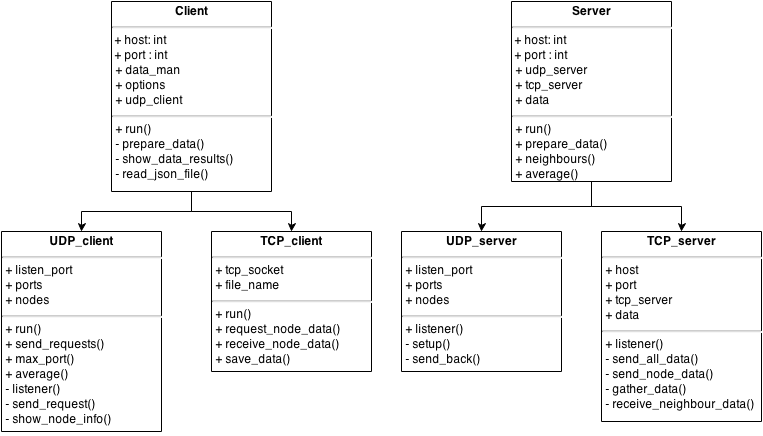
\includegraphics[width=1.0\textwidth]{diagram}
         \\ Fig. 1 Class diagram
      \end{center}
    \end{minipage}
    




  \section{Implementation}

    \subsection{Stored data}

    All information of servers is stored in one single \textit{json} file (\textit{data.json}) in order to reduce redundancy in real project
    each server will have separate file that will contain its specific data.\\

    \textit{JSON} or JavaScript Object Notation, is an open standard format that uses human-readable text to transmit
    data objects consisting of attribute–value pairs. It is used primarily to transmit data between a server and web application, as an alternative to XML. \\

    With this implementation all servers can easily access their data, and thus reduce redundancy in code, and
    optimize the creation and initialization of the servers. The data contains a list of available nodes, more specifically their port number,
    which subsequently contain information about their neigthbours and the list of all employes. \\

    In the code below you can see the the configuration of servers with the information about their neighbours, and list of employers.

    \newpage

    \begin{lstlisting}
    {
      "10000": {
        "neigthbours": [10001],
        "employers":[ ... ]
      },
      "10001": {
        "neigthbours": [10000, 10002],
        "employers":[ ... ]
      },
      "10002": {
        "neigthbours": [10001, 10003],
        "employers":[ ... ]
     },
      "10003": {
        "neigthbours": [10002, 10004],
        "employers":[ ... ]
     },
     "10004": {
        "neigthbours": [10003],
        "employers":[ ... ]
     }
    }
    \end{lstlisting}

    \begin{lstlisting}
    # ...
        "employers":[
            {"firstName":"John",     "lastName":"Doe",       "salary": 150, "department": "Marketing"},
            ...
            {"firstName":"Alex",     "lastName":"Carturari", "salary": 478, "department": "Testing"}
         ]
    # ...
    \end{lstlisting}

    \subsection{Dependencies}

    In the application we used some external packages, (\textit{gems}), that provide
    additional functionality. Below I will provide a small description of each one.

    \begin{itemize}
      \renewcommand{\labelitemi}{$\circ$}
      \item \textit{socket} - provides access to the underlying operating system socket implementations. It can be used to provide more operating system specific functionality than the protocol-specific socket classes.
      \item \textit{json} - allow to generate or parse json easily.
      \item \textit{optparse} -  is a class for command-line option analysis. It is much more advanced, yet also easier to use.
      \item \textit{rainbow} - is a ruby gem for colorizing printed text on ANSI terminals.
      \item \textit{terminal-table} -  is a fast and simple, yet feature rich ASCII table generator written in Ruby.
    \end{itemize}

    \subsection{Client Side}

    The client part of the application is composed of four main file that together provide functionality
    necesary to assure the request to server, receive, save, parse and show the response in form of the
    list of emplyoers from server with the maximum nodes and its neighbours.

    \subsubsection{UDP protocol}

    The class below provides the functionality that assures the transmission
    between server and client using UDP protocol.

    \begin{itemize}
      \renewcommand{\labelitemi}{$\circ$}
      \item  \textit{initialize} - creates a udp socket.
      \item \textit{send\_requests} - method that will send requests to the ports available in its list.
      \item \textit{listener} method serves for receiving udp messages, and store the responses in \textit{@nodes} array,
      that will be used to analyze this information.
      \item \textit{send\_requests} - method that sends request to the ports available in its list for information.
      \item \textit{max\_port} - returns the node with max connections.
      \item \textit{average} - computes the total average of all nodes.
    \end{itemize}


    \begin{lstlisting}
    class UdpClient

      LISTEN_PORT = 20001
      PORTS = [10000, 10001, 10002]

      def initialize host
        BasicSocket.do_not_reverse_lookup = true
        @udp_server = UDPSocket.new
        @udp_server.setsockopt(Socket::SOL_SOCKET,Socket::SO_BROADCAST, true)
        @udp_server.bind(host, LISTEN_PORT)
      end

      def send_requests
        PORTS.each {|port| send_request port}
      end

      def run
        loop {  listener }
      end

      def max_port
        nodes.max_by { |info| info[:neighbours] }[:port]
      end

      def average
        sum = nodes.reduce(0) { |sum, node| sum += node[:average].to_i }
        sum / nodes.size
      end
      private
      def listener
        response, client = @udp_server.recvfrom(1024)
        Thread.new(client) do |clientAddress|
          neighbours, average = response.chomp.split(":")
          nodes << {port: clientAddress[1], neighbours: neighbours, average: average}
          show_node_info(nodes.last)
        end
      end
      # ...
    end
    \end{lstlisting}

    \subsubsection{TCP protocol}

    The class below provides the functionality that assures the transmission
    between server and client using TCP protocol.

    \begin{itemize}
      \renewcommand{\labelitemi}{$\circ$}
      \item \textit{initialize} - First we create a TCP socket, and
      \item \textit{run} - here we call the following methods.
      \item \textit{request\_node\_data} - send a tcp request to receive emplyoers information.
      \item \textit{receive\_node\_data} - receives all information from server.
      \item \textit{save\_data} - saves received data into a file.
    \end{itemize}

    \begin{lstlisting}
    class TcpClient

      def initialize host, file_name, port
        @tcp_socket = TCPSocket.open(host, port)
        @file_name = file_name
      end

      def run
        request_node_data
        save_data(receive_node_data)
      end

      def request_node_data
        tcp_socket.puts "*all*node*data*"
      end

      def receive_node_data
        # ...
      end

      def save_data data
        # ...
      end
    end
    \end{lstlisting}

    \subsubsection{Data manipulation}

    Data manipulation class as the name says it responsible to analyze,
    parse and show received data in a readable form.

    \begin{itemize}
      \renewcommand{\labelitemi}{$\circ$}
      \item \textit{show\_*} - display the information at the console.
      \item \textit{filtered\_data}  - analyze and parse the data.
      \item \textit{table\_format} - add the table format to the parsed data.
    \end{itemize}

    \begin{lstlisting}
    class DataManipulation

      def initialize data, average
        @data = data
        @average = average
      end

      def show_all
        puts table_format(data)
      end

      def show_filtered
        # ...
      end

      private

      def filter_data
        data.select{ |employer| employer["salary"]  > average }
                .sort_by{ |employer| employer["lastName"] }
                .group_by{ |employer| employer["department"] }
      end

      def table_format data
        # ...
      end

    end
    \end{lstlisting}

    \subsubsection{Main}

    The main class \textit{Client} contains all methods that are necesary to start and perform necesary
    work, it also has UDP and TCP functionality by using the  \textit{classes} with the same name.
    Below there is a short description of methods that it has, for the implementation you can see the full code.

    \begin{itemize}
      \renewcommand{\labelitemi}{$\circ$}
      \item In the \textit{contructor} we save provided options and setup udp server.
      \item  \textit{receive\_data} - we setup a tcp server, send requests to servers and save response to a file.
      \item \textit{prepare\_data} - read the json file and initiate the data manipulation class.
      \item \textit{show\_data\_results} - show data received from server, based on option from console.
    \end{itemize}

    \begin{lstlisting}
    class Client

      HOST = 'localhost'
      WAIT_TIME = 3
      FILE_NAME = "client_data.json"

      def initialize options
        @options = options
        @udp_client = UdpClient.new(HOST)
      end

      def run
        # ...
      end

      private

      def receive_data
        tcp_client = TcpClient.new(HOST, FILE_NAME, udp_client.max_port)
        tcp_client.run
      end

      def prepare_data
        data = read_json_file
        @data_man = DataManipulation.new(data, udp_client.average)
      end

      def show_data_results
        case options[:show]
        when "default"   then data_man.show_all
        when "filtered"   then data_man.show_filtered
        else
          puts "Invalid option"
        end
      end

      def read_json_file
        JSON.parse File.read(FILE_NAME)
      end

    end

    # input arguments from terminal
    options = {}
    options[:show] = "default"
    OptionParser.new do |opts|
      opts.banner =  "Usage: ruby client.rb [options]\n\n"
      opts.on("-s", "--show [SHOW]", "show data by method") do |s|
        options[:show] = s || "default"
      end
    end.parse!
    \end{lstlisting}

    One of its most important methods is `run` method, here we first send
    upd request to all servers that this client knows, then after a interval of 3 seconds,
    we close the receiving udp port, and then we establish a tcp connection with the node
    with maximum neighboars, receiving necesary information from it, parse it and show it
    in the console.

    \begin{lstlisting}
    # ...
      def run
        udp_client.send_requests
        begin
          Timeout::timeout(WAIT_TIME) { udp_client.run }
        rescue Timeout::Error => e
          # abort with coupling
          abort("There are no available nodes") if udp_client.nodes.empty?
          p "Port with max connections is #{udp_client.max_port}"

          # save - read - show
          receive_data
          prepare_data
          show_data_results
        end
      end
      # ...
    \end{lstlisting}

    The client actions are started with the following line, it receive
    the actions that need to be applied on the data.

    \begin{lstlisting}
    Client.new(options).run
    \end{lstlisting}

    \subsection{Servers}

    The server part was done by Vasilica Victor but a part of functionality of TCP class was done working together, (pair programming)
    in order to establish the correct connection between servers and client.

    \section{Conclusion}

    In this laboratory work we build a distributed system that has at its basis the different transport protocols TCP and UDP,
    that were used for individual purposes, each doing its own predefined task. Thus after learning more about the advantages
    and disadvantages of each protocol, we apply each to solve their individual task. \\

    At first we used UDP protocol for unicast and multicast transmission in order to receive information related to the number
    of neighbours node of each server (node), and at the same time the average \textit{salary} information. This decision was
    implemented because the \textit{average salary} is represented by a number, and it is easy to send using the udp protocol,
    the downside of this approach is that there is a high chance to lose this data, and this will result in wrong calculation of total
    average of nodes, and represeting the information to the client. \\

    We also worked with \textit{json} in order to store our collection of necesary data, that contains the port number, list of neighboars
    and the list of employers of each node, by reading, parsing and then saving in the same format type. \\

    Thus we learned how to build a small distributed system with a collection of objects using different types of transport protocols. \\

    \textbf{Link to Repository: } \url{https://gitlab.ati.utm.md/petru.negrei/lab2/tree/wip/petru}

   \section{References}

   \begin{itemize}
      \item Ruby Socket \url{http://www.ruby-doc.org/stdlib-1.9.3/libdoc/socket/rdoc/Socket.html}
      \item Ruby TCP  Socket \url{http://www.ruby-doc.org/stdlib-1.9.3/libdoc/socket/rdoc/TCPSocket.html}
      \item Ruby UDP Socket \url{http://ruby-doc.org/stdlib-1.9.3/libdoc/socket/rdoc/UDPSocket.html}
      \item Ruby JSON \url{http://www.ruby-doc.org/stdlib-2.0.0/libdoc/json/rdoc/JSON.html}
      \item Ruby OptionParser \url{http://ruby-doc.org/stdlib-2.1.0/libdoc/optparse/rdoc/OptionParser.html}
   \end{itemize}


\end{document}

